%!TEX root = thesis.tex

\chapter{Literature Review}
\label{chap:literature-review}

Software visualisation is building momentum within the space of live coding. This section seeks to identify the reason for this momentum and identify the purpose and potential for visualisations within this field.

\section{Software}

Understanding changing software has been identified as one of the most important goals within the space of software engineering practice~\cite{Tao2012}. It is the nature of software to change~\cite{Brooks1995} and there is a need for not only the programmer to understand the software but also for knowledge transfer to take place between those modifying the software and those impacted by the changes~\cite{Tao2012}.

Programming languages are the formal languages of software. These languages are typically represented by source code in a plain text format. However, plain text format is limited requiring an interpretation step (parsing and compilation) to acheive a functioning program that can be understood by the computer~\cite{Badros2000}. The same occurs while programming. The programmer needs to comprehend the source code in order to make informed changes. In this case, the programmer conducts the interpretation step within the brain rather than the computer through a process of hypothesis creation, confirmation and refinement~\cite{Brooks1983}.

The steps involved in and the issues with interpreting and comprehending source code have been comprehensively examined within the literature (see ~\cite{Novais2013,McLean2010a,Brooks1995,Desmond,Rajlich2002}). Nevertheless, although many studies discuss the limitations of text-based source code, comparatively few have conducted empirical user studies examining the effectiveness of alternative representations of source code.

The concept of alternative source code representations is not new. Alternative representations of the source code include diagrams~\cite{Rumbaugh2004}, visual languages~\cite{Cox2007} and combinations of the two (e.g.~\cite{Lucanin2011}). Modern software development environments may also include tools that allow for alternative representations of code~\cite{Cox2007}. Diagrams, visual languages and modern software development environments vary greatly in the relation to the source code with visualiasations representing many levels of abstraction~\cite{Jerding1997}. Despite the differences in the level of abstraction and goal of the alternative representations, these approaches are all related through their common use of visualisation techniques.

\section{Visualisation}

Visualisation is widely understood as ``the use of computer-supported, interactive, visual representations of data to amplify cognition''~\cite{Card1999}. Further extensions of this definition discuss the need to perform cognitive work more efficiently~\cite{Ware2013a} and the need to transfer knowledge~\cite{Burkhard}. These definitions are summarised in the model shown in Figure~\ref{fig:model-of-visualisation}.

\begin{figure}
  \centering 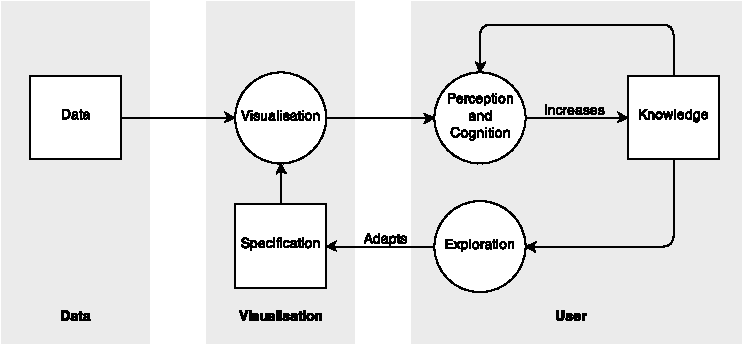
\includegraphics[width=\columnwidth]{../images/diagrams/wijk-model-of-visualisation.pdf}
  \caption[Generic model of visualisation]{Generic model of visualisation \protect\cite{VanWijk2005}.}
\label{fig:model-of-visualisation}
\end{figure}

Software visualisation is the process of representing the characteristics of computer programs visually~\cite{Stasko1992} in order to improve understanding~\cite{Diehl2007}. The advantage of providing a visual representation over the more traditional text-based representation is that the text-based approach does not take full advantage of human visual information processing capabilities~\cite{Myers1989}.

Initial efforts to classify software visualisations identified two axes: whether the visualisation illustrated the code, the data or the algorithm and whether the visualisation was static or dynamic~\cite{Myers1989}. Taxonomies characterised software visualisations according to the aspect of the program, the abstractness of the visualisation, the animation and the automation of the visualisation~\cite{Stasko1992}.

Although it is the nature of software to change, static diagrams have traditionally been used to represent software systems visually. These diagrams typically show the structure (class diagrams) or function (state diagrams) of a software system at a specific moment in time~\cite{Rumbaugh2004}. The usefulness of these diagrams lies in their ability to represent fundamental structures within the program more concisely than the source code itself. However, it is not possible to represent a program's behaviour using these types of static diagrams~\cite{Baecker1998} and it is difficult to represent the evolution of the software using nothing but static diagrams.

% Visual languages provide an alternative method of interaction with the software development process. However, visual languages are often not suited to general purpose programming~\cite{Myers1989}, providing only a subset of a full-featured text-based language.

Approaches to dealing with the visualisation of software evolution and realtime feedback have been integrated into modern software development environments. Modern software development systems usually consist of an \ac{IDE} to manipulate source code. These systems may feature syntax highlighting to assist in comprehension~\cite{Chen2005,Reis}, source code annotations, the generation of visualisations based on the source code~\cite{Hendrix2004} and allow the programmer to interact with the running program. These modern \acp{IDE} emphasise the relationship between the source code and the running program but are still fundamentally tools for source code manupulation. 

Only the initial steps have been taken in order to implement and evaluate methods of communicating source code intent outside the field of programmer comprehension. Studies hint at the limitations of static diagrams, visual languages and modern software development environments and identify the need for alternative software reprentations and evaluation of their effectiveness for those with limited programming knowledge and experience. 

Visualisations have the capacity to present information more effectively than traditional programming languages. Nevertheless, software visualisations still require significant development to benefit in the understanding of the complexity of software ~\cite{Baecker1995}. Effective software visualisations contribute to making software easier to understand, reflecting the software's history through the lifecycle, facilitating the transfer of knowledge from the programmer to the observer, making important structures visible and managing software complexity~\cite{Baecker1995}.

% how have others implemented visualisations into other fields... what have been the strategies, how successful has it been, what are the general guidelines...

In a process-oriented activity such as live coding, different code visualisation techniques are necessary~\cite{McLean2010a,Magnusson2013}. However, these academic treatments of code visualisation in live coding adopt a survey-based approach, and the techniques discussed have not been subject to empirical evaluation. {\color{red} use this paragraph to link to the next section}

\section{Live Coding}

\begin{figure}
\centering
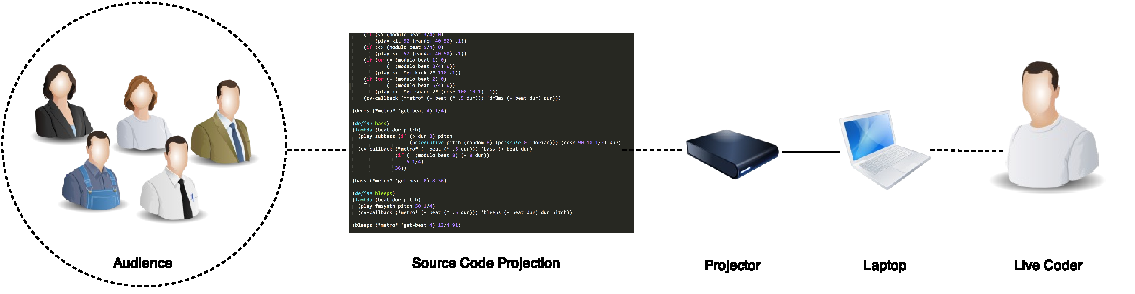
\includegraphics[width=1.0\textwidth]{../images/live-coding-setup.pdf}
\caption[The live coding process]{Conceptual diagram of the live coding process.}
\label{fig:live-coding-setup}
\end{figure}

Live coding can be broadly defined as writing a program while it runs~\cite{Ward2004}. More specifically, live coding is identified as the artistic process of musical and visual expression through programming~\cite{Collins2003}. Figure~\ref{fig:live-coding-setup} shows the standard live coding setup.

The live coding programming practice emphasises the concept of \emph{liveness}, a concept covered comprehensively within the literature~\cite{Auslander,Masura2007}. Liveness is foundational to the performance aspect of live coding in which the mantra is ``show us you screens'', asserting that all live coders should display their raw program source code to the audience.

A unique oportunity is provided through live coding to combine both source code and software visualisation techniques~\cite{McLean2010a}. This is due to the approach of live coding involving effective sensory communication, a goal of transparency of the coding process, and direct manipulation and refinement of the running program.

Firstly, live coding is built around communicating visually and audibly. This extends beyond the physical process of programming. Human input is visible in the creative process, demonstrating a link between physical actions and artistic output \cite{Mclean}. Studies of live coding regarding the effects of visual and audible communication have indicated... \more

Secondly, live coding has a history exposing audiences to code with the goal of live coding to ensure the transparency of the coding process~\cite{Collins2011,McLean2010a}. It provides a space in which there is a direct mapping from the human interaction with the source code to the musical or visual output~\cite{Mclean}. This relationship allows for visuals to map the interaction with the output.

Lastly, live coding allows for direct manipulation and refinement of the running program~\cite{Swift2013}. This provides the capacity for uninterrupted visualisation of the dynamic aspects of the program combined with the static nature of the source code. Similarly, manipulation and refinement of the running program allows for manipulation of the software visualisation~\cite{McLean2010a}.
%- what does this achieve?
%- how do visualisations apply... what can they achieve within this space

% {\color{red} Studies conducted into the communication of the live coding process suggest that audiences may have a sense of exclusion from the live coding performance.}

\section{Programmer and Observer}

The relationship between the programmer and the observer has significant implications not just within the field of live coding but also within software engineering practice.

Commonly within live coding, the live coding artist is performing in front of an audience to entertain or educate. This setup includes the live coder as the programmer and the audience as a passive observer. Similar structures occur within software engineering practice in pair programming~\citetemp{x}. In this case, rather than a passive role, the observer takes the active role of communicating mistakes or considering new ideas.

The similarity between the observer within live coding and the observer within pair programming is that both observers are required to perform a task: understanding the code as the programmer is writing it.

{\color{red} why is this pair programming stuff relevant?}

Audiences are yet to be surveyed as to whether the projected code within a live coding performance gives a greater sense of communication between the programmer and observer or a greater sense of alienation~\cite{Mclean2011}. Similarly, studies are yet to be conducted to determine if source code is the best way of communicating the programming process.

\more

\section{Enjoyment and Understanding}

There is currently a search for software visualisations that increase enjoyment and understanding~\cite{McLean2010a}. Here enjoyment refers to the perceived benefit gained from observing the visualisations regardless of the level of understanding. Understanding refers to the ability of an observer or audience to comprehend the abstract thinking process of the programmer.

Enjoyment is the most common reaction to the positive effect of media~\cite{Vorderer2004}. Increasing enjoyment is one of the fundamental goals of the modern media entertainment industry and with increased enjoyment usually characterised by ``pleasurable affective response to a stimulus''~\cite{Brock2004}.

Enjoyment results in increased attention to the stimulus and has been suggested to increase learning outcomes~\citetemp{x}. \more
% -how do these factors relate to understanding?\\
% -how do these factors relate to visualistions?\\
% -how can these two factors contribute to effective visualisations?\\
% -the concept assignment problem~\cite{Biggerstaff1994}

Understanding of a particular program is said to be achieved when the program can be explained ``in terms that are qualitatively different from the tokens used to construct the source code''~\cite{Biggerstaff1994}. Source code comprehension has a large body of research both within the understanding of text-based source code~\citetemp{x} and within the space of software visualisation~\cite{Hosking2005}.

In the space of live coding, this understanding is required to avoid a sense of distraction or exclusion~\cite{McLean2010a}. Furthermore, understanding software while it is changing presents an additional challenge~\cite{Eisenbarth2003}.

Understanding and enjoyment are often considered opposite concepts when implementing strategies to increase one or the other. 
% -enjoyment is not completely separable from understanding. (not dual?)\\
% -why can we not separate the two?\\
% -what is the duality?\\
% -how does this relate to visualisations?

-Expressiveness vs Effectiveness \cite{Hundhausen2002,Hundhausen1996} \more

\section{Didacticism and Aestheticism}

Enjoyment and understanding are often closely associated with the concepts of didacticism and aestheticism.

Didacticism refers to the ultimate goal of teaching. This approach mirrors the concept of understanding from the previous section. A didactic approach intends to increase the level of understanding.
% -what is didacticism?\\
% -how does it relate to visualisations?\\
% -how does it relate to education?

Aestheticism refers to the ultimate goal of appealing to the senses. This approach mirrors the concept of enjoyment from the previous section. An aesthetic approach intends to increase visualisation usability and increase retention~\cite{Cawthon2007}. Live coding has much potential and opportunity to evaluate and improve aesthetic effect~\cite{Bell}.

% The artistic nature of the live coding field cannot be ignored when evaluating the effect of aesthetic and didactic approaches on the enjoyment and understanding of the audience.
% -how does it relate to art?\\
% -why is it still a good approach for evaluating understanding.

Software visualisations within the space of live coding have the potential to manipulate these two variables~\cite{Iru,McLean2010a}. For example, by increasing visual interest it may be possible to increase aesthetic appeal. Though increasing aesthetic appeal may reduce didacticism with increased visual complexity causing confusion.

The educational aspects of software visualisations have been examined in a number of studies~\citetemp{x} though few have applied these visualisations to areas outside of the field of software engineering and fewer still have investigated software visualisations targeted at those with no programming experience.

There has been an initial examination of the aesthetics in graph drawing~\citetemp{x} and within the space of software graph visualsations~\citetemp{x}, though no studies have examined the effectiveness of process-driven software visualisations. This is particularly the case for the examination of live coded visualisations and the effect on audiences.

Some frameworks for both aesthetic evaluation of visualisations~\cite{Cawthon2007,Purchase1996} and didactic evaluation of visualisations~\cite{VanWijk2005} have been developed though a thorough evaluation of the combination of the two concepts has not been considered.

\section{Future Directions}

The literature raises a number of questions and identifies a number of limitations with the current state of research in the visualisation of live code.

There are suggestions that it may be possible to combine or balance the goals of didacticism and aestheticism in order to manipulate understanding and enjoyment~\citetemp{x}.

Regarding the visualisation of live coding, the most important questions identified include how can visualisations be applied to live coding and what should be used as the metric to measure the success of the application of visualisations. Furthermore, the the limitations of the current methods of software visualisation in general have been identified including how to best visualise the process of programming, how to visualise the evolution of software~\cite{Gall1999} and how to improve understanding and enjoyment of programming.

Reviewing the model in Figure~\ref{fig:model-of-visualisation} from the didactic and aesthetic perspective identifies some limitations. Within this model, a gain in knowledge is the only measurement of value and the only identified method for increased cognitive performance and increased exploration. The literature has identified a need to redefine the model of software visualisation with a goal of increasing the dimensions of understanding and enjoyment and didacticism and aestheticism~\citetemp{x}.

The literature identifies some gaps in the current understanding of live coding. Questions raised include, ``why show the source code at all during a live coding performance?'' and ``are there better methods of demonstrating the programming process?''. Systematic and empirical studies are yet to be conducted within live coding to answer these questions. Similarly, although metrics for evaluating visualisations~\citetemp{x}, no studies have been conducted to evaluate effective metrics for analysis of the live coding process and the display of source code or visuals.

To attempt to answer some of these questions, these limitations within the literature were to be investigated in an exploratory field study in an effort to define the direction of the development and implementation of software visualisations within live coding.

